\documentclass[14pt,a4paper]{article}
\usepackage{amsmath,amssymb,physics}
\usepackage{graphicx}
\usepackage{siunitx}
\usepackage{bm}
\usepackage{geometry}
\geometry{margin=2.5cm}
\makeindex
\DeclareUnicodeCharacter{2009}{}
\DeclareUnicodeCharacter{2061}{}
\DeclareUnicodeCharacter{2212}{}
\DeclareUnicodeCharacter{200B}{}

\title{Moment of Inertia and Angular Momentum in Astrophysics}
\author{Francesco Lazzarotto \& ChatGPT}
\date{2026-02-20}

\begin{document}

\maketitle

\begin{abstract}
 In this article we'll show physics concepts as Moment of Inertia and Angular Momentum and how we can see them in astrophysical systems and phenomena, like planets and stars motion and orbits. Equation and formulas that describe them will be shown and explained.
\end{abstract}
\begin{figure}[!ht]
\begin{center}
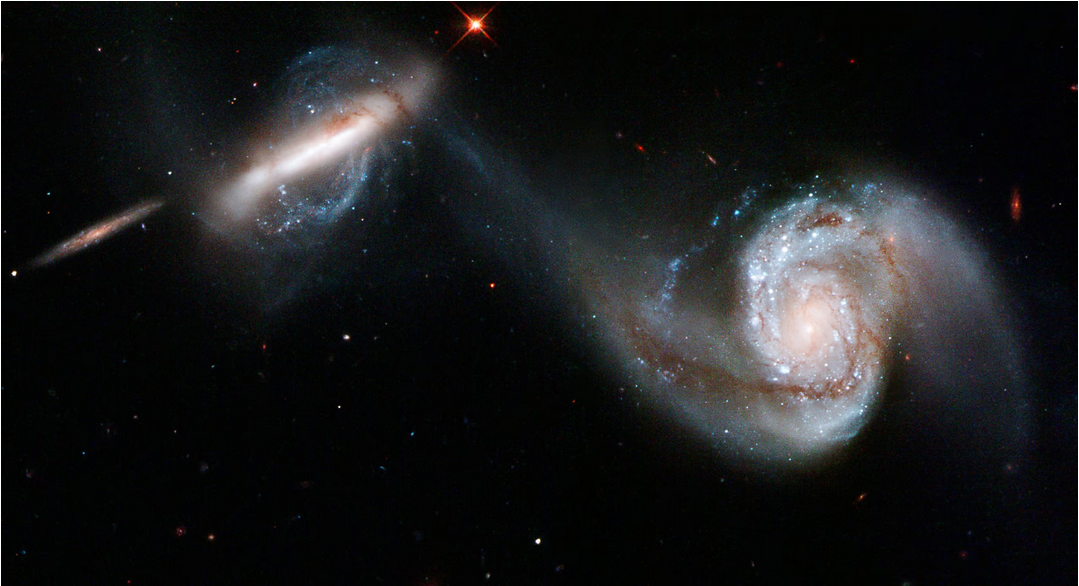
\includegraphics[width=0.7\textwidth]{orbiting_galaxies.png}
\caption{Orbiting Galaxies}
\end{center}
\end{figure}
\clearpage
\tableofcontents
\clearpage

\section{General Framework}
We work in plane polar coordinates for a central-force problem. In a central force problem (like gravity),
\begin{itemize}
\item Angular momentum is conserved,
\item Motion is confined to a plane.
\end{itemize}
Therefore, we usually reduce the problem to 2D polar coordinates in that plane. Mathematically \(\vb{r}(t)\) is a vector in 3 Dimensions:
\[
\vb{r}(t) \in R^3
\]
but dynamically it evolves in a fixed plane.
More precisely:\\
\begin{itemize}
\item r(t) is a scalar function of time (the radial distance)\\
\item \(\hat{\vb{r}}\) is the radial unit vector, which depends on the angle \(\theta(t)\)\\
\end{itemize}

So explicitly:

\[ r(t)=r(t)\hat{\vb{r}}(t) \]

Important point:

\[ \hat{\vb{r}}=\cos\theta(t) \hat{\vb{i}} + \sin\theta(t)\hat{\vb{j}}\]

So the unit vector itself depends on time, because
\(\theta=\theta(t)\). This is the fundamental geometric point.\\

\[r(t)=|\vb{r}(t)|\]

r(t) is the magnitude of the position vector.\\ So:
\begin{itemize}
\item \( r(t) \rightarrow \) scalar
\item \( \vb{r}(t) \rightarrow \) vector
\item \( \hat{\vb{r}}(t) \rightarrow \) unit vector
\end{itemize}
This is equivalent to writing in Cartesian coordinates:
\[ r(t)=x(t)\hat{\vb{i}}+y(t)\hat{\vb{j}} \]
but polar coordinates align with the physics.\\
For a point mass $m$ orbiting a central mass $M$:

\[
\vb{r}(t) = r(t)\,\hat{\vb{r}}, \qquad
\vb{v}(t) = \dot{r}\hat{\vb{r}} + r\dot{\theta}\hat{\vb{\theta}}
\]
where
\[
 r(t)\,\hat{\vb{r}}
\]
\[(scalar)\times(unit\,vector)\]

We differentiate:

\[ \vb{r}(t) = r(t)\,\hat{\vb{r}} \]

Using product rule:

\[ v=\dot{r}\hat{\vb{r}}+r\dot{\hat{\vb{r}}} \]

Now here is the key geometric identity:

\[ \dot{\hat{\vb{r}}} = \dot{\theta} \hat{\vb{\theta}} \]

So:

\[ v=\dot{r}\hat{\vb{r}}+r \dot{\theta} \hat{\vb{\theta}} \]

This shows:
\begin{itemize}
\item First term \(\rightarrow\) radial velocity
\item Second term \(\rightarrow\) transverse (angular) velocity
\end{itemize}

In the orbital plane the radial unit vector is:

\[ \hat{\vb{r}} = \cos⁡\theta \hat{\vb{i}} + sin⁡\theta \hat{\vb{j}} \]

The transverse (angular) unit vector is:

\[ \hat{\vb{\theta}} = -sin⁡\theta\hat{\vb{i}} + \cos⁡\theta\hat{\vb{j}} \]

These two vectors:
\begin{itemize}
\item have unit magnitude,
\item are orthogonal,
\item rotate with angle \(\theta\)
\end{itemize}

Differentiate \( \hat{\vb{r}} \)
Since  \( \theta = \theta(t) \) , apply the chain rule:

\[
\frac{d}{dt}\hat{\vb{r}} =  \frac{d}{dt}
\begin{pmatrix}
\cos\theta\\
\sin\theta\\
\end{pmatrix}
\]
\[
=
\begin{pmatrix}
-\sin\theta\dot{\theta}\\
 \cos\theta\dot{\theta}\\
\end{pmatrix}
\]

Factor out \(\dot{\theta}\):
\[
=
\dot{\theta}
\begin{pmatrix}
-\sin\theta\\
\cos\theta\\
\end{pmatrix}
\]
But this vector is exactly:
\[ \hat{\vb{\theta}} \]
Therefore:

\[
\boxed{
\dot{\hat{\vb{r}}}=\dot{\theta}\hat{\vb{\theta}}
}
\]

The magnitude of \( \hat{\vb{r}} \) is constant:

\[ |\hat{\vb{r}}|=1 \]

Differentiate:
\[
\frac{d}{dt} (\hat{\vb{r}} \cdot \hat{\vb{r}}) = 0
\]
\[
2\hat{\vb{r}}\dot{\hat{\vb{r}}} = 0
\]
So:
\[
\hat{\vb{r}}\dot{\hat{\vb{r}}} = 0
\]
This proves that the derivative is perpendicular to \(\hat{\vb{r}}\).\\
The only perpendicular direction available in the plane is \(\hat{\vb{\theta}}\)\\
The magnitude must be proportional to angular speed \(\dot{\theta}\)\\
So geometrically:
\begin{itemize}
\item The unit vector does not change length.
\item It only rotates.
\item Its rate of change is purely tangential.
\end{itemize}
This is identical to uniform circular motion of a unit vector.
\section{Visual demonstration}
\begin{figure}[!ht]
\begin{center}
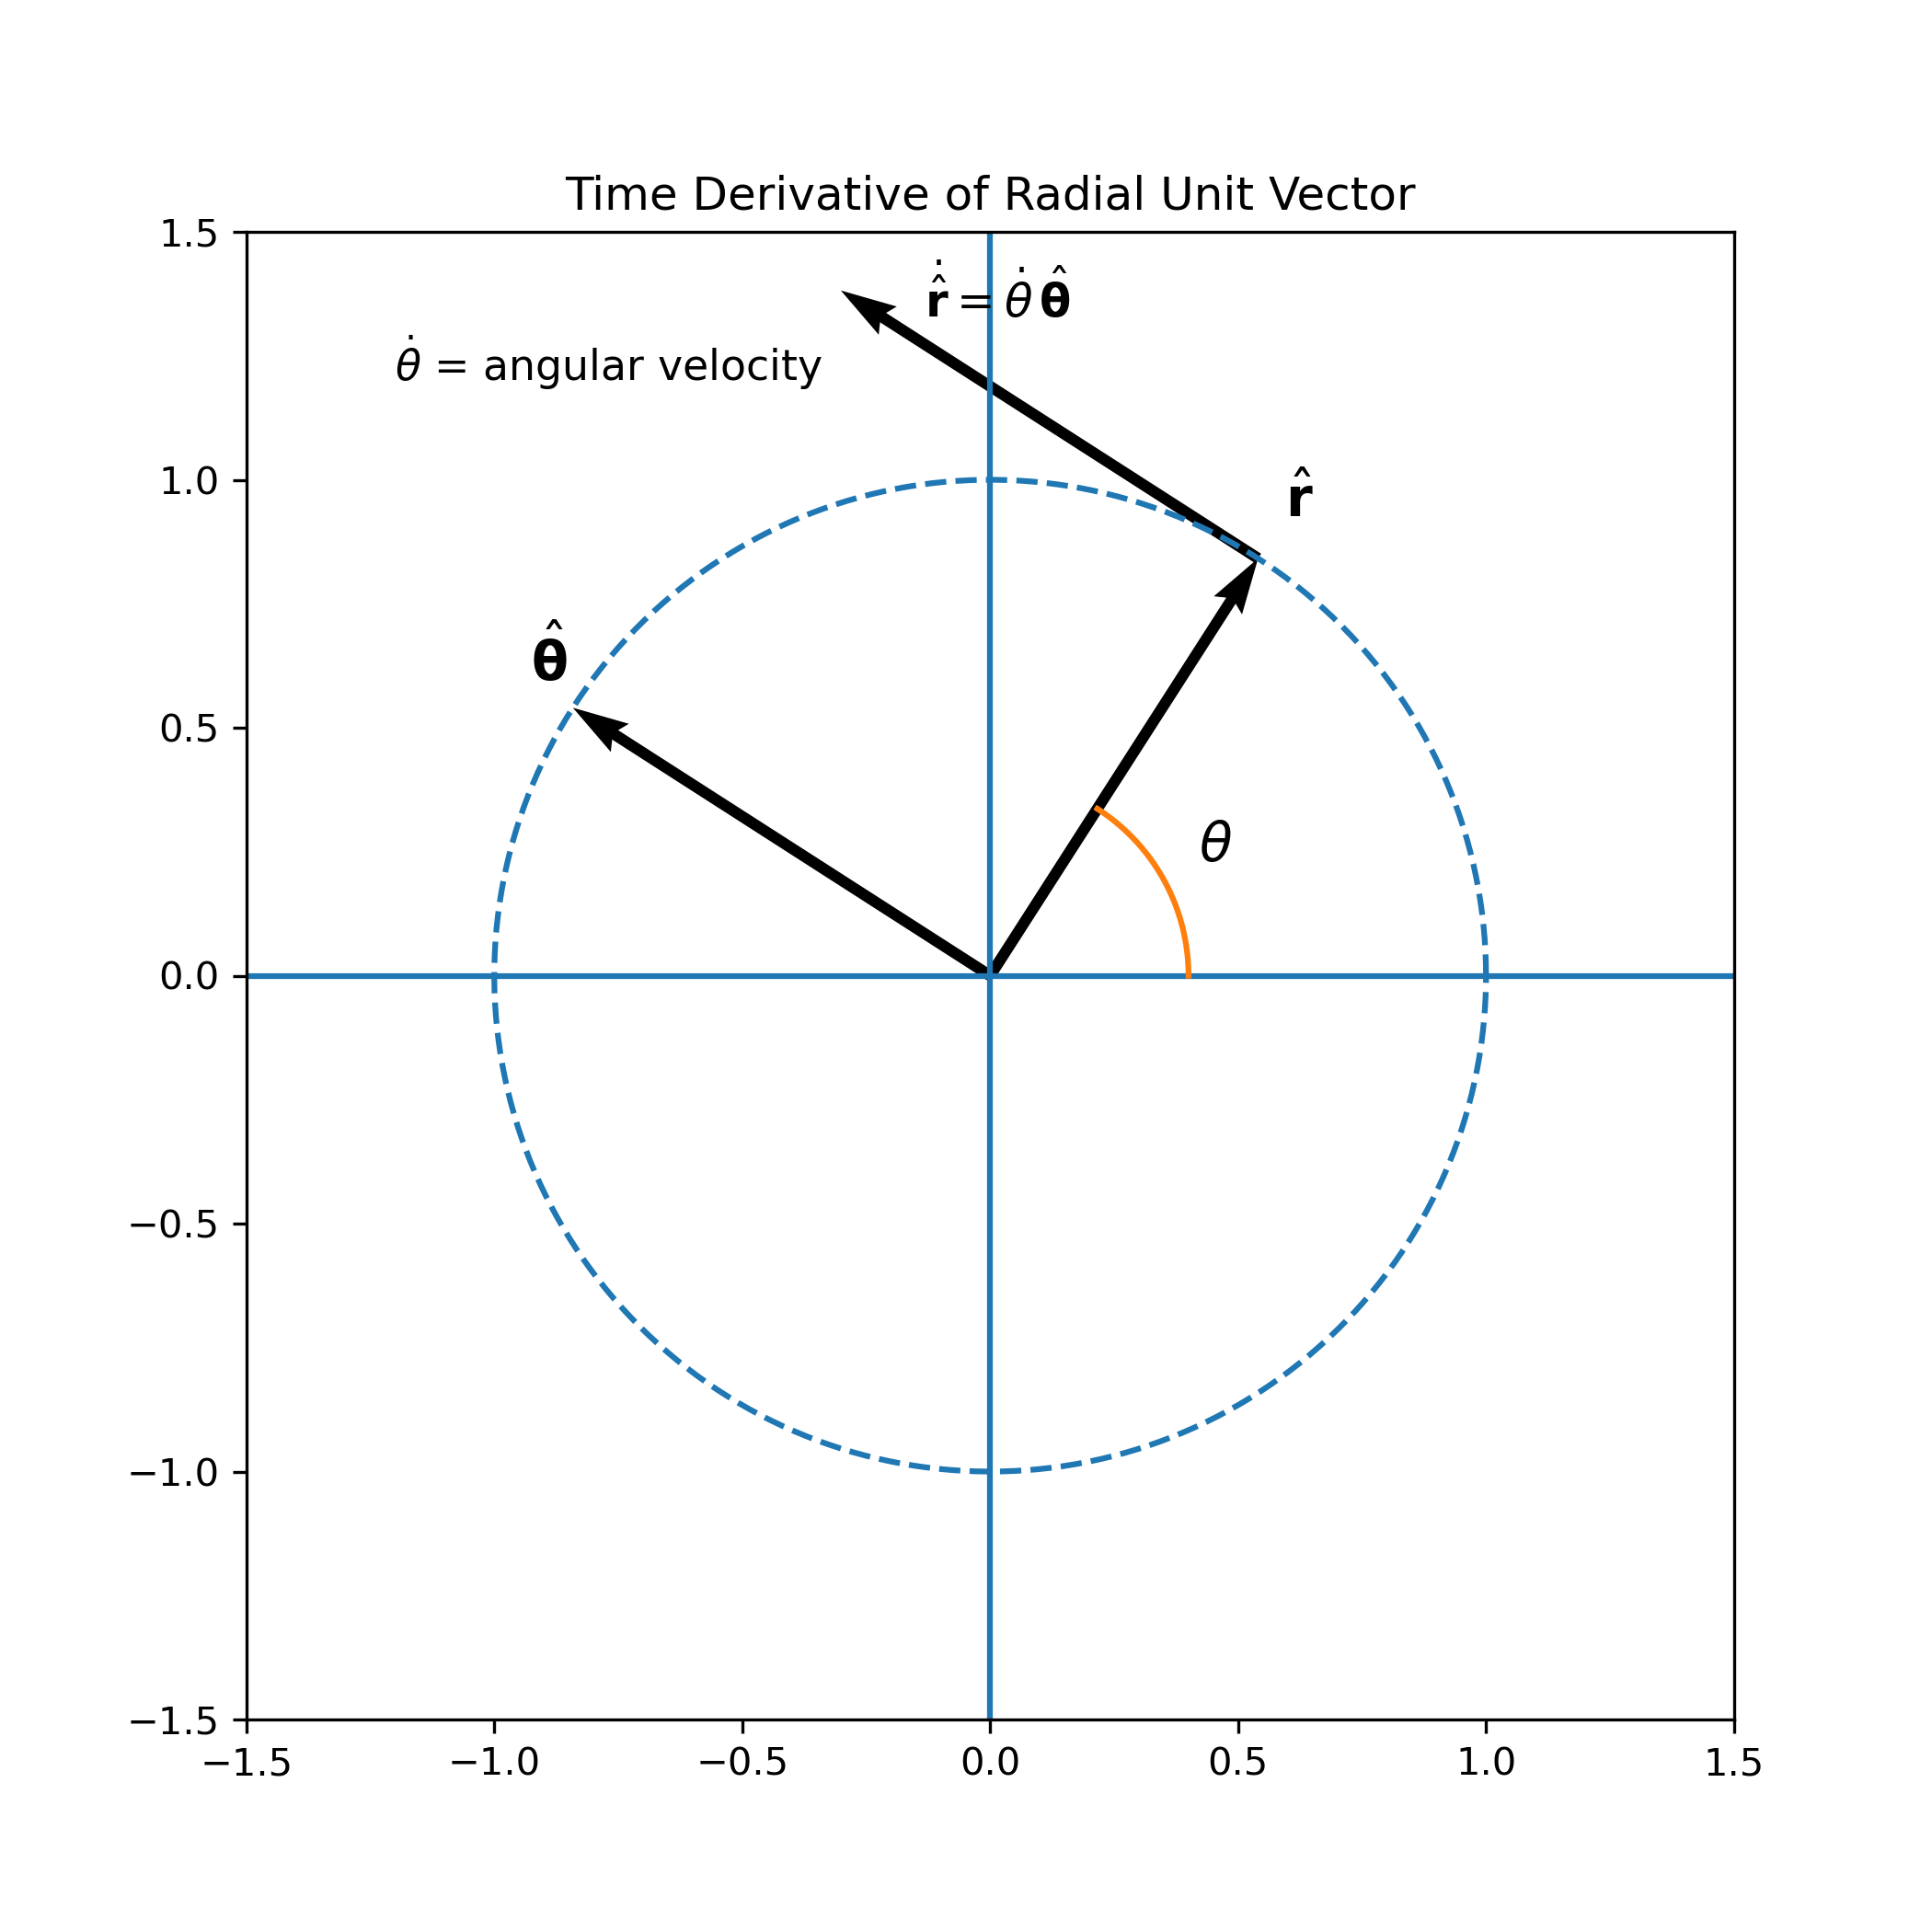
\includegraphics[width=0.7\textwidth]{unit_vector_derivative.png}
\caption{Unit vector derivative}
\end{center}
\end{figure}
\flushbottom
The script below:
\begin{itemize}
\item Draws \(\hat{\vb{r}}\)
\item Computes its time derivative numerically,
\item Shows that the derivative vector aligns with \(\hat{\vb{\theta}}\).
\end{itemize}
Save as: \verb|unit_vector_derivative.py|
\begin{verbatim}
import numpy as np
import matplotlib.pyplot as plt

# Time parameter
t = 1.0

# Angular speed
omega = 1.0

# Angle
theta = omega * t

# Unit radial vector
r_hat = np.array([np.cos(theta), np.sin(theta)])

# Unit theta vector
theta_hat = np.array([-np.sin(theta), np.cos(theta)])

# Analytical derivative
dr_hat_dt = omega * theta_hat

# Plot
plt.figure()

# Draw unit circle
angles = np.linspace(0, 2*np.pi, 500)
plt.plot(np.cos(angles), np.sin(angles))

# Draw vectors
plt.quiver(0,0,r_hat[0],r_hat[1], angles='xy', scale_units='xy', scale=1)
plt.quiver(r_hat[0],r_hat[1],dr_hat_dt[0],dr_hat_dt[1],
           angles='xy', scale_units='xy', scale=1)

plt.quiver(0,0,theta_hat[0],theta_hat[1],
           angles='xy', scale_units='xy', scale=1)

plt.gca().set_aspect('equal')
plt.xlim(-1.5,1.5)
plt.ylim(-1.5,1.5)

plt.title("Derivative of Radial Unit Vector")
plt.savefig("unit_vector_derivative.png")
plt.show()
\end{verbatim}
Angular momentum:
\[
\vb{L} = \vb{r} \times m\vb{v}
\]

For circular motion ($r=\text{const}$):
\[
L = m r^2 \omega = m r v
\]

Equation of motion (Newtonian gravity):

\[
m\ddot{\vb{r}} = -\frac{GMm}{r^3}\vb{r}
\]

For circular orbit:

\[
\omega^2 = \frac{GM}{r^3}
\]

Moment of inertia of extended body:

\[
I = \int r^2 \, dm
\]

Uniform solid sphere:

\[
I = \frac{2}{5}MR^2
\]

Angular momentum of rotating sphere:

\[
L = I\omega
\]

%---

\section{Example 1: Earth Orbiting the Sun}

Parameters:

\[
M_\odot = 1.989\times10^{30}\,\text{kg}
\]
\[
m_\oplus = 5.972\times10^{24}\,\text{kg}
\]
\[
r = 1\,\text{AU} = 1.496\times10^{11}\,\text{m}
\]

Orbital velocity:

\[
v = \sqrt{\frac{GM_\odot}{r}} \approx 29.8\,\text{km/s}
\]

Angular velocity:

\[
\omega = \frac{v}{r}
\]

Angular momentum:

\[
L = m_\oplus r v
\]

Displacement vector:

\[
\vb{r}(t) = r(\cos\omega t\,\hat{\vb{i}} + \sin\omega t\,\hat{\vb{j}})
\]

\section{Python Script to Generate Orbit Figure}

Here the script \verb|earth_orbit.py|:

\begin{verbatim}
import numpy as np
import matplotlib.pyplot as plt

r = 1.0
theta = np.linspace(0, 2*np.pi, 500)

x = r*np.cos(theta)
y = r*np.sin(theta)

plt.figure()
plt.plot(x, y)
plt.scatter(0,0)
plt.gca().set_aspect('equal')
plt.xlabel('x')
plt.ylabel('y')
plt.title('Circular Orbit')
plt.savefig("earth_orbit.png")
plt.show()
\end{verbatim}

%---
\begin{figure}[!ht]
\begin{center}
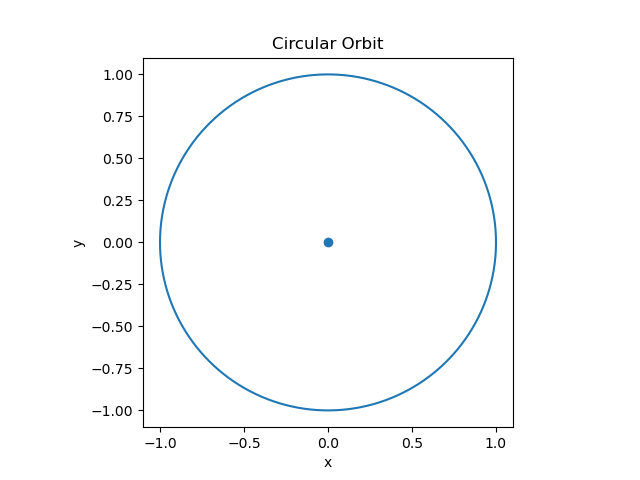
\includegraphics[width=0.7\textwidth]{earth_orbit.png}
\caption{Earth Orbit}
\end{center}
\end{figure}
\flushbottom
%---

\section{Example 2: Earth's Rotation (Moment of Inertia)}

Earth radius:

\[
R_\oplus = 6.371\times10^6\,\text{m}
\]

Moment of inertia (approximate solid sphere):

\[
I = \frac{2}{5} m_\oplus R_\oplus^2
\]

Angular velocity:

\[
\omega = \frac{2\pi}{T}
\]

with $T=86164\,\text{s}$ (sidereal day).

Rotational angular momentum:

\[
L = I\omega
\]

%---

\section{Example 3: Star Orbiting a Supermassive Black Hole}

Example: star orbiting a SMBH of mass

\[
M = 4\times10^6 M_\odot
\]

Orbital equation (Keplerian ellipse):

\[
r(\theta) = \frac{a(1-e^2)}{1 + e\cos\theta}
\]

Angular momentum per unit mass:

\[
h = \sqrt{GMa(1-e^2)}
\]

Total angular momentum:

\[
L = m h
\]

\subsection*{Python Script for Elliptical Orbit}

\begin{verbatim}
import numpy as np
import matplotlib.pyplot as plt

a = 1
e = 0.7
theta = np.linspace(0, 2*np.pi, 1000)
r = a*(1-e**2)/(1+e*np.cos(theta))

x = r*np.cos(theta)
y = r*np.sin(theta)

plt.figure()
plt.plot(x,y)
plt.scatter(0,0)
plt.gca().set_aspect('equal')
plt.title('Elliptical Orbit')
plt.savefig("elliptical_orbit.png")
plt.show()
\end{verbatim}

\begin{figure}[!ht]
\begin{center}
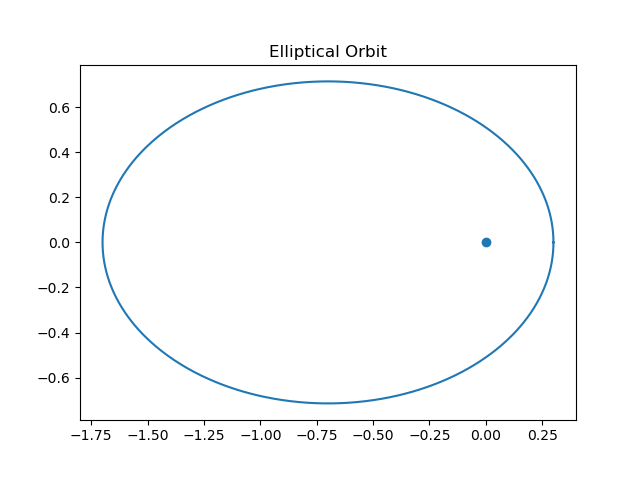
\includegraphics[width=0.7\textwidth]{elliptical_orbit.png}
\caption{Elliptical Orbit}
\end{center}
\end{figure}
\flushbottom
%---
\section{Example 4: Galaxy Rotation}

For a star orbiting inside a galaxy:

\[
v(r) = \sqrt{\frac{GM(r)}{r}}
\]
where \(M(r)\) = mass enclosed within radius r\\

This comes from Newton's Shell Theorem:\\

For a spherically symmetric mass distribution:
\begin{itemize}
\item Mass outside radius r exerts no net gravitational force.
\item Only mass inside radius r contributes.
\end{itemize}
So the gravitational acceleration is:
\[a(r)=\frac{GM(r)}{r^2}\]​
For circular orbit:
\[ \frac{v^2}{r}=\frac{GM(r)}{r^2}\]
Multiply both sides by r:
\[ v^2=\frac{GM(r)}{r} \]
So:
\[\boxed{v(r)=\sqrt{\frac{GM(r)}{r}}}\]
\subsubsection{Physical Interpretation}
The behavior of v(r) depends entirely on how M(r) grows with radius.
Let’s analyze cases.
\begin{itemize}
\item Case A — Solar System (central mass only)
If almost all mass is concentrated at the center:
\[M(r) \approx M = constant\]
Then:
\[v(r)\propto\frac{1}{\sqrt{r}}\]
This is called \textbf{Keplerian decline}.\\
Velocity decreases with distance.\\
That is what we observe in the Solar System.\\
\item Case B — Uniform density sphere\\
If density is constant:
\[ \rho = const \]
Then:
\[M(r)=\frac{4}{3}\pi r^3 \rho \]
Plug in:
\[v(r)=\sqrt{\frac{G\frac{4}{3}\pi r^3 \rho}{r}}\]
\[v(r)\propto r\]
So velocity increases linearly.\\
This is like a solid-body rotation.\\
\item Case C — Flat Rotation Curve (Observed in Galaxies)

Observations show:\\
\[v(r) \approx constant\]
Let’s call it \(v_0\).
Then:
\[v_0^2=\frac{GM(r)}{r}\]
Solve for mass:
\[M(r)=\frac{v_0^2}{G}r\]
So:
\[ \boxed{M(r)\propto r} \]
\end{itemize}
That is shocking.\\
Mass keeps increasing linearly with radius.\\
This implies:
\begin{itemize}
\item There must be unseen mass.
\item That mass extends far beyond the visible disk.
\end{itemize}
This is the dark matter evidence.
\subsubsection{Units in Galaxies}
Typical spiral galaxy values:
\begin{itemize}
\item Radius: 1–30 kpc
\item \(1\, kpc = 3.086 \times 10^{19} m\)
\item Velocity: ~200 km/s
\end{itemize}
So a realistic plot would have:
\begin{itemize}
\item r in kiloparsecs
\item v in km/s
\end{itemize}
A realistic curve has three regions:
\begin{enumerate}
\item Inner bulge \(\rightarrow\) solid body rotation \( v \propto r \)
\item Transition region
\item Outer flat region  \( v \approx constant\)
\end{enumerate}
If Newtonian gravity holds:
\begin{itemize}
\item Flat velocity means M(r) must grow indefinitely.
\item But visible matter does not.
\end{itemize}
Hence:
\begin{itemize}
\item Dark matter halo.
\end{itemize}
if density behaves as:
\[\rho(r) \propto \frac{1}{r^2}\]
Then:
\[M(r) \propto r\]
And:
\[v(r)=constant\]
This density profile appears in isothermal sphere models.\\
Observed flat rotation curves:
\[
v(r) \approx \text{constant}
\]

Implies:

\[
M(r) \propto r
\]

Angular momentum of star:

\[
L = m r v
\]

\subsection*{Python Script for Rotation Curve}

\begin{verbatim}
import numpy as np
import matplotlib.pyplot as plt

r = np.linspace(0.1, 10, 500)
v = np.ones_like(r)

plt.figure()
plt.plot(r, v)
plt.xlabel("r")
plt.ylabel("v")
plt.title("Flat Galaxy Rotation Curve")
plt.savefig("rotation_curve.png")
plt.show()
\end{verbatim}
\begin{figure}[!ht]
\begin{center}
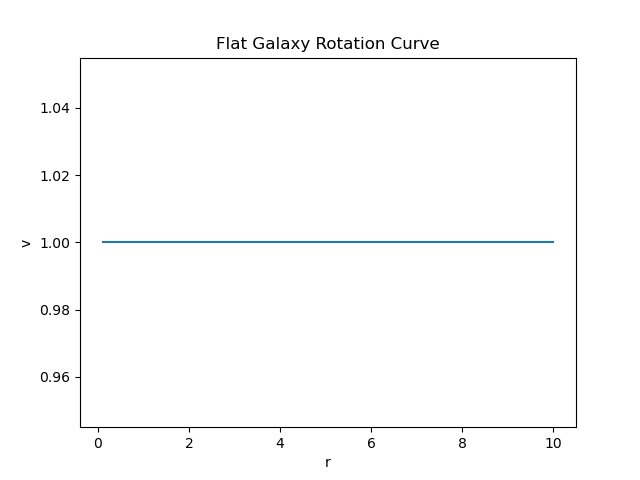
\includegraphics[width=0.7\textwidth]{rotation_curve.png}
\caption{Flat Galaxy Rotation Curve}
\end{center}
\end{figure}
\flushbottom
%---
We'll show now a physically meaningful galaxy rotation curve script with:
\begin{itemize}
\item Real units:
\begin{itemize}
\item Radius in kpc
\item Velocity in km/s
\end{itemize}
\item Three cases:
\begin{itemize}
\item Central point mass (Keplerian decline)
\item Uniform density sphere (solid-body rise)
\item Dark matter halo (flat curve)
\end{itemize}
\item Proper labels, legend, grid
\item Physically reasonable Milky-Way–like parameters
\end{itemize}
\subsubsection{Physical Model}
We use:
\[v(r)=\sqrt{\frac{GM(r)}{r}}\]
We will define three enclosed-mass models:
\begin{itemize}
\item Case 1 — Central Mass (Keplerian)
\[ M(r)=M_0 \]
Typical galactic bulge mass:
\[ M_0=5\times10^{10}M_\odot \]
Velocity decreases as:
\[ v\propto r^{-1/2} \]
\item Case 2 — Uniform Density Sphere
\[M(r)=\frac{4}{3}\pi \rho r^3\]
Velocity grows linearly:
\[v \propto r\]
\item Case 3 — Dark Matter Halo (Isothermal Sphere)
We impose:
\[v(r) \rightarrow 0 \]
Typical:
\[v_0=220\,km/s\]
Then:
\[M(r)=\frac{v_0^2}{G}r\]
\end{itemize}
Constants Used
\begin{itemize}
\item \(G = 6.67430\times10^{−11} m^3/kg/s^2\)
\item \(1\,kpc=3.086\times10^{19} m\)
\item \(1\,M_\odot=1.989\times10^{30} kg\)
\end{itemize}
\begin{figure}[!ht]
\begin{center}
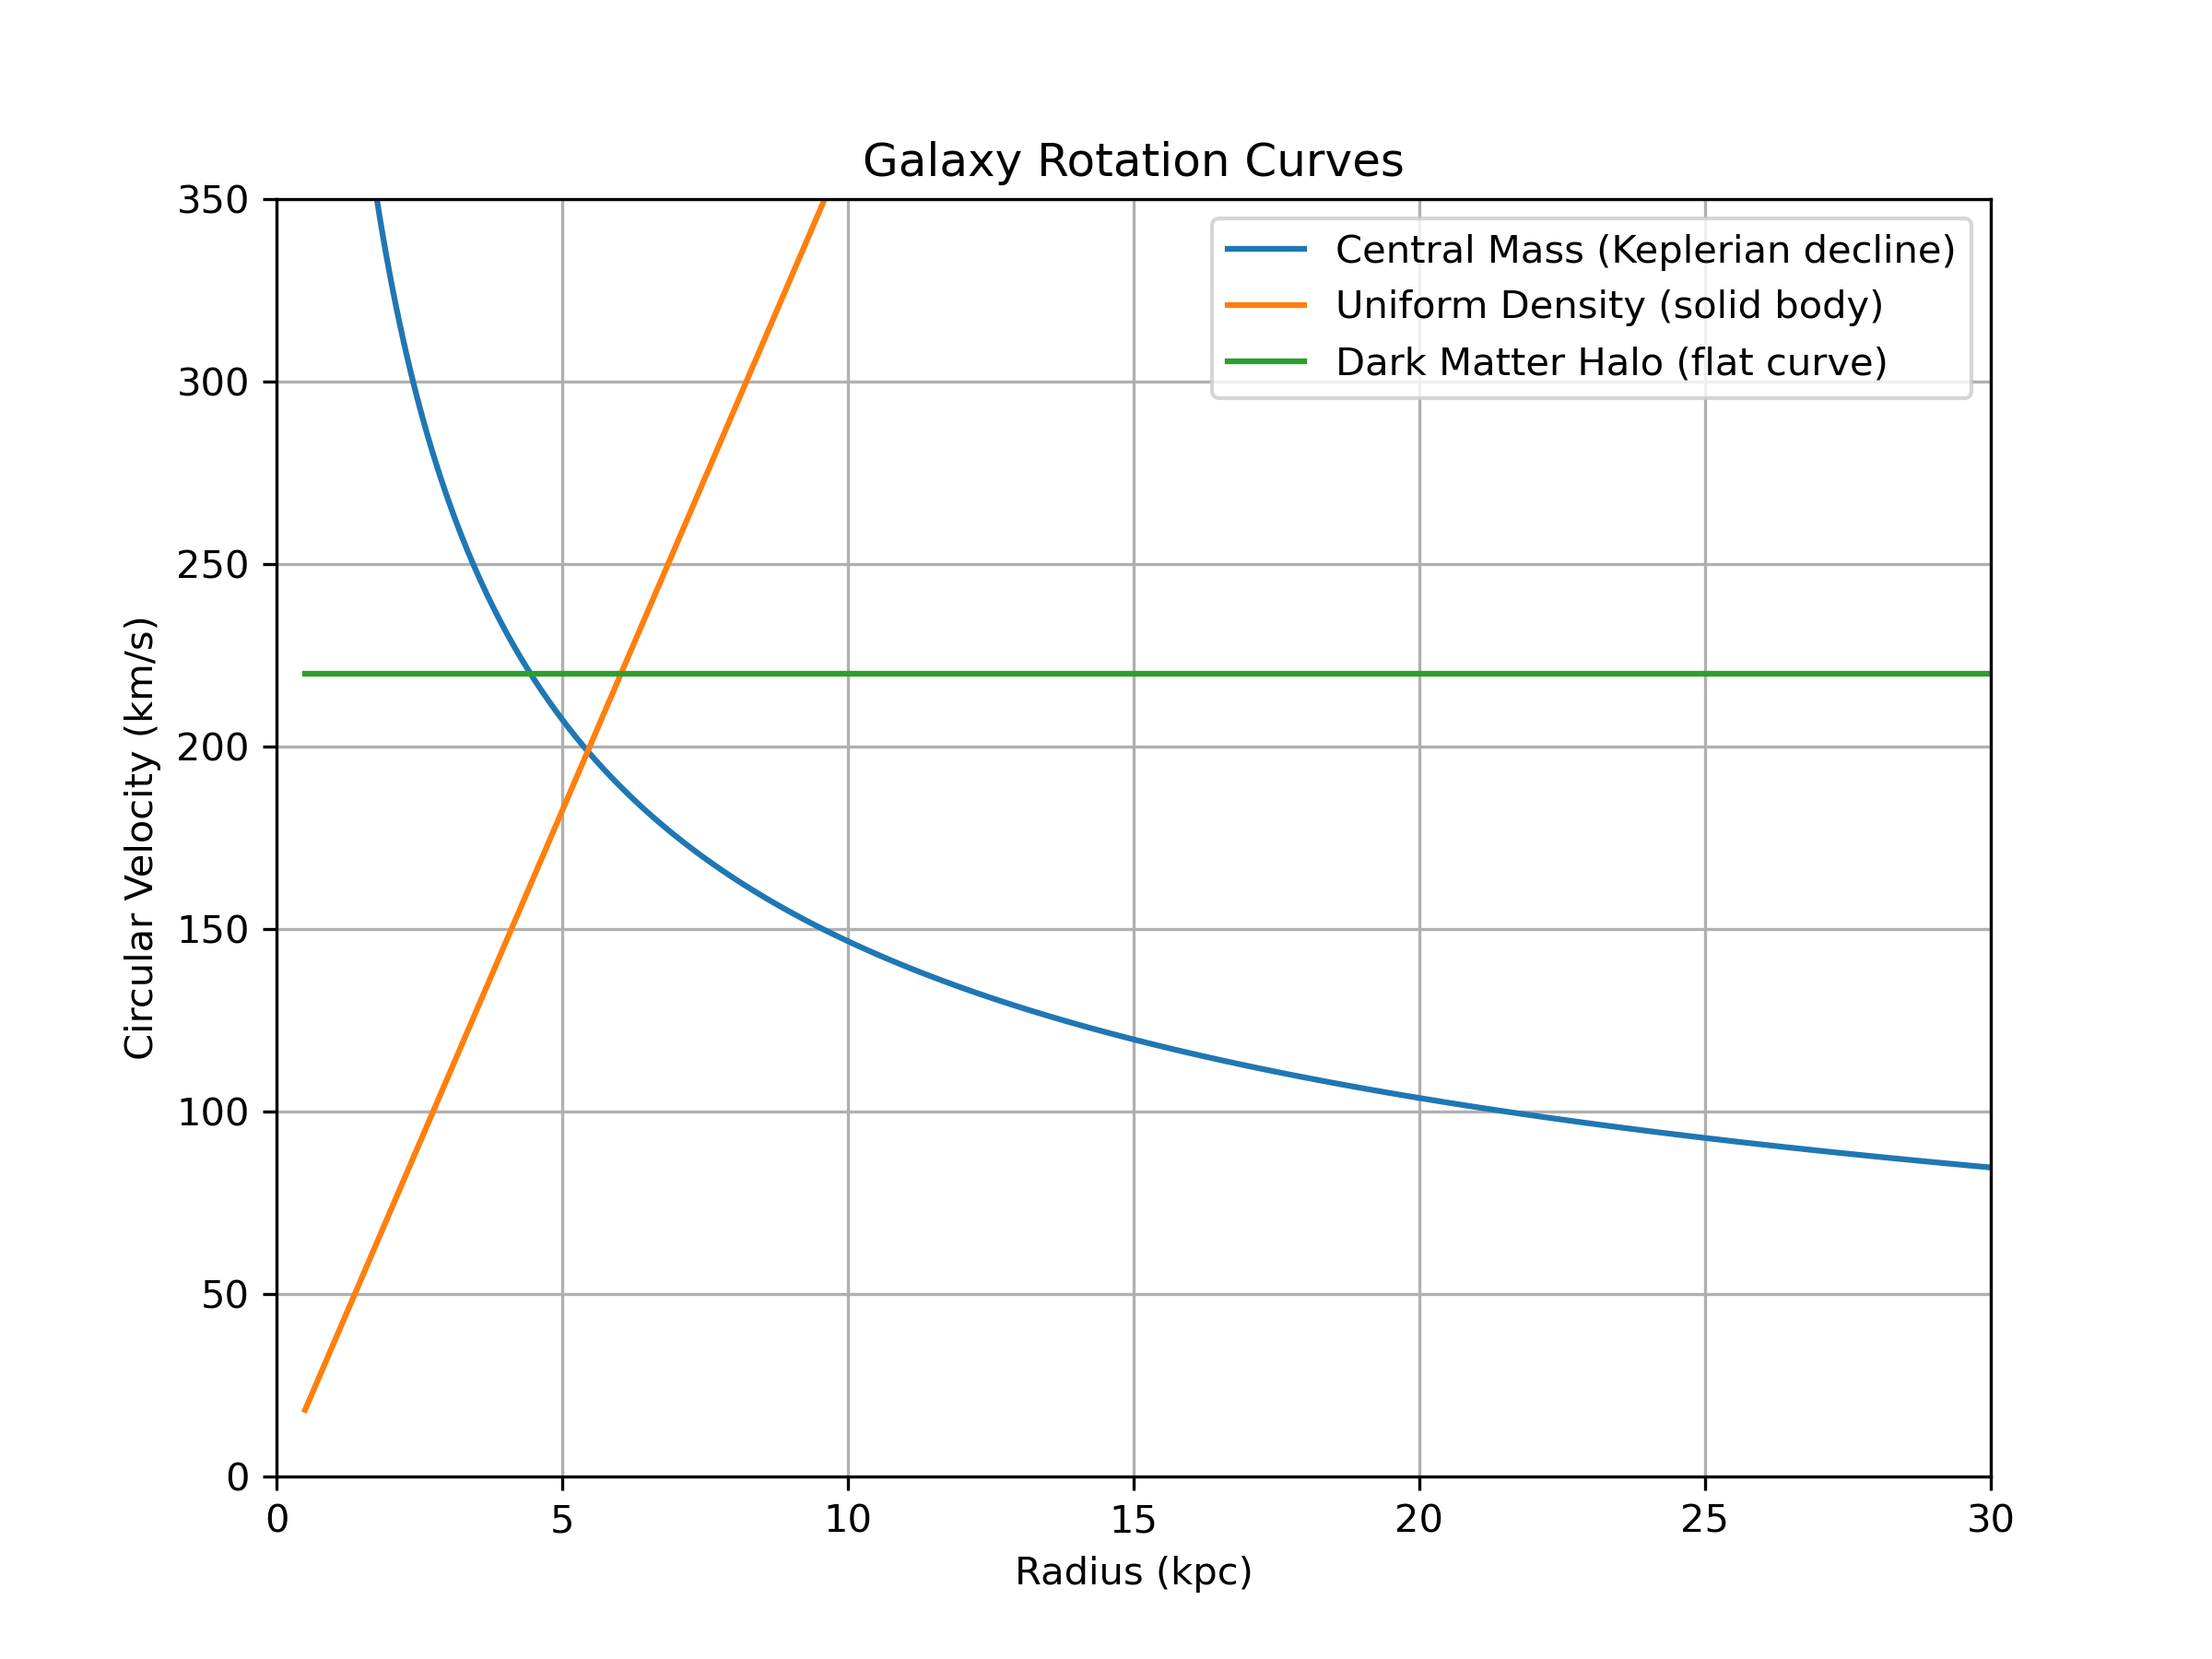
\includegraphics[width=0.7\textwidth]{real_rotation_curves.png}
\caption{Galaxy Rotation Curves}
\end{center}
\end{figure}
\flushbottom
\textbf{Python Script (Real Units)}\\
Save as: \verb|real_rotation_curve.py|
\begin{verbatim}
import numpy as np
import matplotlib.pyplot as plt

# Physical constants
G = 6.67430e-11            # m^3 kg^-1 s^-2
Msun = 1.989e30           # kg
kpc = 3.086e19            # meters

# Radius range (kpc)
r_kpc = np.linspace(0.5, 30, 500)
r_m = r_kpc * kpc

# -----------------------------
# Case 1: Central mass
# -----------------------------
M0 = 5e10 * Msun
v_kepler = np.sqrt(G * M0 / r_m) / 1000  # km/s

# -----------------------------
# Case 2: Uniform density sphere
# -----------------------------
rho = 5e-21  # kg/m^3 (chosen to give realistic velocities)
M_uniform = (4/3) * np.pi * rho * r_m**3
v_uniform = np.sqrt(G * M_uniform / r_m) / 1000  # km/s

# -----------------------------
# Case 3: Flat rotation curve (dark halo)
# -----------------------------
v0 = 220  # km/s
v_flat = np.ones_like(r_kpc) * v0

# -----------------------------
# Plot
# -----------------------------
plt.figure(figsize=(8,6))

plt.plot(r_kpc, v_kepler, label="Central Mass (Keplerian decline)")
plt.plot(r_kpc, v_uniform, label="Uniform Density (solid body)")
plt.plot(r_kpc, v_flat, label="Dark Matter Halo (flat curve)")

plt.xlabel("Radius (kpc)")
plt.ylabel("Circular Velocity (km/s)")
plt.title("Galaxy Rotation Curves")
plt.legend()
plt.grid(True)

plt.xlim(0, 30)
plt.ylim(0, 350)

plt.savefig("real_rotation_curves.png", dpi=300)
plt.show()
\end{verbatim}
What You Will See
\begin{itemize}
\item Blue curve: decreasing \(v \propto r^{−1/2}\)
\item Orange curve: rising \(v \propto r\)
\item Green horizontal line: flat curve (~220 km/s)
\end{itemize}
Physical Interpretation of the Plot
\begin{table}[h!]
\begin{center}
\begin{tabular}{|c|c|c|}
\hline
\textbf{Region}& \textbf{Dominant Physics}& \textbf{Behavior}\\
\hline
Inner bulge& Stellar mass& $v \propto r$\\
\hline
Intermediate& Transition& Peak velocity\\
\hline
Outer halo& Dark matter& $v \propto constant$\\
\hline
\end{tabular}
\end{center}
\caption{Galaxy physical model}
\end{table}
\textbf{Important Note}:\\
The uniform-density model is unrealistic at large radius — it is just pedagogical.\\
Real galaxies combine:\\
\begin{itemize}
\item Bulge
\item Stellar disk (exponential profile)
\item Dark matter halo (NFW or isothermal)
\end{itemize}
\subsubsection{observational galactic dynamics}.
The velocities of stars at different galactocentric radii have been measured, and they lie approximately on the flat rotation curve (~220–240 km/s for the Milky Way disk). But there is an important distinction:
\begin{itemize}
\item Disk stars \(\rightarrow\) follow circular rotation curve
\item Halo stars \(\rightarrow\) do not (they have random, non-circular orbits)
\item S-stars near the central black hole \(\rightarrow\) Keplerian regime
\end{itemize}
So different stellar populations lie on different dynamical regimes.
How Are Velocities Measured?\\
For Milky Way stars we use:
\begin{enumerate}
\item Radial velocity\\
From Doppler shift (spectroscopy)
\item Proper motion\\
From astrometry (e.g., ESA's Gaia mission)
\end{enumerate}
Combining:
\[ v=\sqrt{v_r^2+v_t^2} \]
where transverse velocity:
\[v_t=4.74 \mu d\]
with:
\begin{itemize}
\item \(\mu\) in arcsec/year
\item d in parsec
\item velocity in km/s
\end{itemize}
The Milky Way Rotation Curve (Observed)\\
At the Sun's location:
\[R_0\approx 8.2\,kpc\]
Circular velocity:
\[ v_0\approx230\,km/s\]
Observations show:
\begin{itemize}
\item 5-20 kpc \(\rightarrow\) roughly flat
\item \(<\)2 kpc \(\rightarrow\) rising
\item 20 kpc \(\rightarrow\) still approximately flat (within uncertainties)
\end{itemize}
\clearpage
\subsubsection{Example Stars at Different Radii}
Below is a representative list of well-studied objects.\\
\textbf{Important!}:\\
For most individual stars, the total velocity relative to the Galactic center is measured, but only disk stars follow circular motion closely.
\begin{enumerate}
\item The Sun
\begin{itemize}
\item Galactocentric distance: 8.2 kpc
\item Circular velocity: ~230 km/s
\item Lies on flat part
\end{itemize}
\item HD 17925 (thin disk star)
\begin{itemize}
\item Distance: ~8 kpc
\item Velocity: ~220 km/s (rotational component)
\item Lies on flat curve
\end{itemize}
\item Cepheid variables (outer disk tracers)
Typical example:
\begin{itemize}
\item Distance: 12-15 kpc
\item Velocity: 210-230 km/s
\item Still on flat curve
\end{itemize}
These are often used to trace the disk rotation.
\item Outer HI gas clouds (not stars but key tracers)
\begin{itemize}
\item Distance: 20-25 kpc
\item Velocity: ~200-220 km/s
\item Clearly flat regime
\item Gas is actually the best tracer of rotation curves.
\end{itemize}
\item S2 star (near central black hole)
\begin{itemize}
\item Distance: ~0.005 pc (~0.0000015 kpc)
\item Pericenter velocity: ~7600 km/s
\item Follows Keplerian curve
\item Dominated by central black hole mass
\end{itemize}
This is not on flat curve — this is pure central mass regime.
\item Halo star (example: SDSS J102915+172927)
\begin{itemize}
\item Distance: ~8–15 kpc
\item Velocity: 300+ km/s
\item Does NOT follow circular rotation
\item Random orbit (halo population)
\end{itemize}
Halo stars do not define rotation curve.
\end{enumerate}
\clearpage
Summary Table
\begin{table}[h!]
\begin{center}
\begin{tabular}{|c|c|c|c|}
\hline
\textbf{Object Type}& \textbf{Radius (kpc)}& \textbf{Velocity (km/s)}& \textbf{Regime}\\
\hline
S2 (near SMBH)&	~0.0000015&	~7600&	Keplerian\\
\hline
Inner bulge stars&	1–2& 100–200& Rising\\
\hline
Sun& 8.2& ~230& Flat\\
\hline
Disk stars& 5–15& 210–240& Flat\\
\hline
HI gas (outer)& 20–25& ~200& Flat\\
\hline
Halo stars& 5–50& 100–400& Non-circular\\
\hline
\end{tabular}
\end{center}
\caption{Galaxy Objects Motion}
\end{table}
\begin{figure}[!ht]
\begin{center}
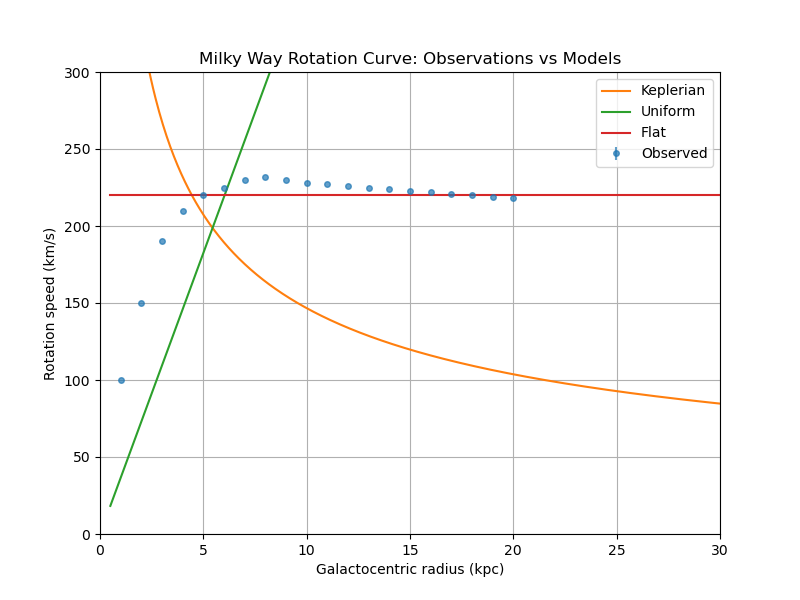
\includegraphics[width=0.7\textwidth]{ObservedRotation.png}
\caption{Observed Rotation vs model}
\end{center}
\end{figure}
\flushbottom
\section{Gnuplot Alternative (Circular Orbit)}
\begin{verbatim}
set terminal png
set output "orbit.png"
set parametric
set trange [0:2*pi]
plot cos(t), sin(t)
\end{verbatim}

\begin{figure}[!ht]
\begin{center}
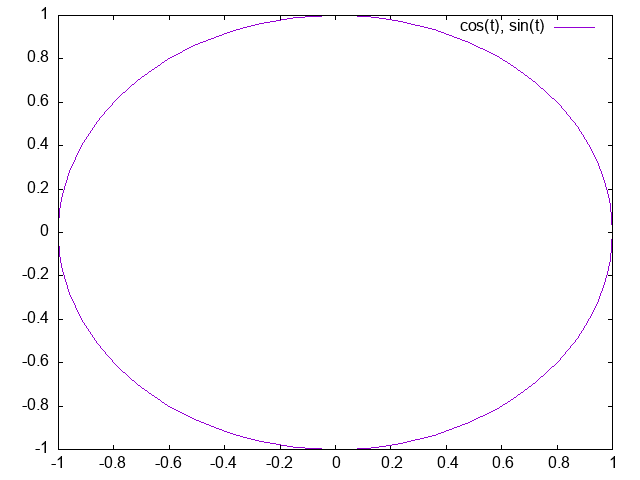
\includegraphics[width=0.7\textwidth]{orbit.png}
\caption{gnuplot Elliptical Orbit}
\end{center}
\end{figure}
\flushbottom

%---

\section{Equation of Motion in Vector Form}

Full Newtonian two-body equation:

\[
\ddot{\vb{r}} = -\frac{GM}{r^3}\vb{r}
\]

Conservation of angular momentum:

\[
\frac{d\vb{L}}{dt} = 0
\]

Conservation of energy:

\[
E = \frac{1}{2}mv^2 - \frac{GMm}{r}
\]

%---



\section{The Newtonian Two-Body Problem}

Consider two masses $m_1$ and $m_2$ interacting gravitationally. Their equations of motion are:

\[
m_1 \ddot{\vb{r}}_1 = -\frac{G m_1 m_2}{|\vb{r}_1 - \vb{r}_2|^3}(\vb{r}_1 - \vb{r}_2)
\]
\[
m_2 \ddot{\vb{r}}_2 = -\frac{G m_1 m_2}{|\vb{r}_2 - \vb{r}_1|^3}(\vb{r}_2 - \vb{r}_1)
\]

\subsection{Reduction to One-Body Problem}

Define:

\[
\vb{R} = \frac{m_1 \vb{r}_1 + m_2 \vb{r}_2}{m_1 + m_2}
\quad\text{(center of mass)}
\]

\[
\vb{r} = \vb{r}_1 - \vb{r}_2
\quad\text{(relative coordinate)}
\]

The total motion separates into:

\[
\ddot{\vb{R}} = 0
\]

\[
\mu \ddot{\vb{r}} = -\frac{G m_1 m_2}{r^3} \vb{r}
\]

where:

\[
\mu = \frac{m_1 m_2}{m_1 + m_2}
\]

is the reduced mass.

Thus, the two-body problem reduces to a single particle of mass $\mu$ moving in a central potential:

\[
V(r) = -\frac{G m_1 m_2}{r}
\]

\section{Lagrangian Formalism}

The Lagrangian in polar coordinates is:

\[
L = T - V
\]

\[
T = \frac{1}{2}\mu \left( \dot{r}^2 + r^2 \dot{\theta}^2 \right)
\]

\[
V = -\frac{G m_1 m_2}{r}
\]

Hence:

\[
L = \frac{1}{2}\mu \left( \dot{r}^2 + r^2 \dot{\theta}^2 \right)
+ \frac{G m_1 m_2}{r}
\]

Since $\theta$ does not appear explicitly in $L$, it is a cyclic coordinate.

From Euler–Lagrange equations:

\[
\frac{d}{dt} \left( \frac{\partial L}{\partial \dot{\theta}} \right) = 0
\]

\[
\frac{\partial L}{\partial \dot{\theta}} = \mu r^2 \dot{\theta}
\]

Thus:

\[
\mu r^2 \dot{\theta} = \text{constant} = h
\]

This is conservation of angular momentum.

\section{Effective Potential}

Radial equation becomes:

\[
\mu \ddot{r} = -\frac{d}{dr} \left( -\frac{G m_1 m_2}{r} + \frac{h^2}{2\mu r^2} \right)
\]

Define effective potential:

\[
V_{\text{eff}}(r) = -\frac{G m_1 m_2}{r}
+ \frac{h^2}{2\mu r^2}
\]

Interpretation:
\begin{itemize}
\item First term: gravitational attraction.
\item Second term: centrifugal barrier.
\end{itemize}
Circular orbits satisfy:

\[
\frac{dV_{\text{eff}}}{dr} = 0
\]

leading to:

\[
r = \frac{h^2}{\mu G m_1 m_2}
\]

\section{Orbit Equation}

Using substitution $u = 1/r$:

\[
\frac{d^2 u}{d\theta^2} + u = \frac{G(m_1+m_2)}{h^2}
\]

Solution:

\[
r(\theta) = \frac{p}{1 + e\cos\theta}
\]

with:

\[
p = \frac{h^2}{\mu G (m_1+m_2)}
\]

This is the conic section solution:
\begin{itemize}
\item $e<1$ ellipse
\item $e=1$ parabola
\item $e>1$ hyperbola
\end{itemize}
\section{Moment of Inertia Tensor}

For extended astrophysical bodies (stars, planets), rotation is described by:

\[
I_{ij} = \int \rho(\vb{r})
\left( r^2 \delta_{ij} - x_i x_j \right) d^3 r
\]

Properties:

- Symmetric tensor
- Can be diagonalized in principal axes
- Angular momentum:

\[
L_i = I_{ij} \omega_j
\]

For spherical symmetry:

\[
I_{ij} = \frac{2}{5}MR^2 \delta_{ij}
\]

Real stars are not perfectly uniform; differential rotation modifies $I$.

\section{Virial Theorem in Astrophysics}

For gravitational systems:

\[
2\langle T \rangle + \langle V \rangle = 0
\]

For bound systems:

\[
E = T + V = -T = \frac{1}{2}V
\]

Implications:
\begin{itemize}
\item Galaxies
\item Star clusters
\item Dark matter mass estimation
\end{itemize}
\section{Angular Momentum in Galaxies}

Specific angular momentum:

\[
j = \frac{L}{M}
\]

Observed scaling relation:

\[
j \propto M^{2/3}
\]

Interpretation:

Galactic angular momentum arises from tidal torques in early structure formation.

\section{General Relativistic Correction}

In Schwarzschild metric, orbit equation becomes:

\[
\frac{d^2 u}{d\theta^2} + u =
\frac{GM}{h^2} + 3GM u^2
\]

Small correction leads to perihelion precession:

\[
\Delta \theta =
\frac{6\pi GM}{a(1-e^2)c^2}
\]

Explains Mercury's anomalous precession.

\section{Physical Interpretation Summary}

\begin{itemize}
\item Angular momentum conservation arises from rotational symmetry (Noether theorem).
\item Central gravitational forces produce planar motion.
\item Effective potential explains orbital stability.
\item Moment of inertia tensor governs rotational dynamics of extended bodies.
\item Virial theorem connects kinematics and gravitational binding.
\item Relativistic corrections become important near compact objects.
\end{itemize}

\section{Further Numerical Exploration (Python Example)}
\begin{figure}[!ht]
\begin{center}
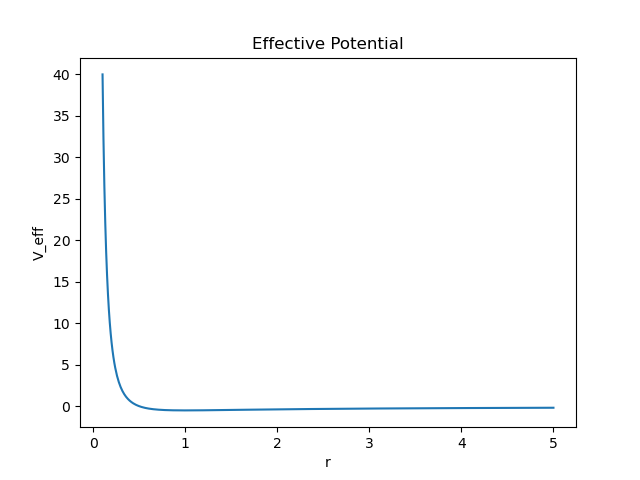
\includegraphics[width=0.7\textwidth]{effective_potential.png}
\caption{Effective Potential}
\end{center}
\end{figure}
\flushbottom

Example: Effective potential plot.

\begin{verbatim}
import numpy as np
import matplotlib.pyplot as plt

G = 1
M = 1
mu = 1
h = 1

r = np.linspace(0.1,5,500)
Veff = -G*M/r + h**2/(2*mu*r**2)

plt.figure()
plt.plot(r,Veff)
plt.xlabel("r")
plt.ylabel("V_eff")
plt.title("Effective Potential")
plt.savefig("effective_potential.png")
plt.show()
\end{verbatim}

\section{Summary}

Astrophysical systems illustrated:

\begin{itemize}
\item Orbital angular momentum $L = mr^2\omega$
\item Rotational angular momentum $L = I\omega$
\item Keplerian motion from inverse-square law
\item Galactic rotation requiring extended mass distribution
\end{itemize}

\end{document}



